% !TEX TS-program = pdflatex
% !TEX encoding = UTF-8 Unicode

\documentclass[UTF8, a4paper, 12pt]{report}
	\title{模式识别作业\\——Fisher分类器}
	\author{姓名学号}
	\date{2020/12/22}

\usepackage{ctex}
\usepackage{amsmath}
\usepackage{amssymb}
\usepackage{titlesec} % set Chapter1 to chinese 第一章
\usepackage{zhnumber}
\titleformat{\chapter}{\raggedright\Huge\bfseries}{第\,\zhnum{chapter}\,章}{1em}{}
 \usepackage{indentfirst} % 首行缩进
\usepackage{enumitem} % 序号
\usepackage{graphicx} % 插图
\makeatletter
\newcommand*\bigcdot{\mathpalette\bigcdot@{.5}}
\newcommand*\bigcdot@[2]{\mathbin{\vcenter{\hbox{\scalebox{#2}{$\m@th#1\bullet$}}}}}
\makeatother

\usepackage[noend]{algpseudocode}
\usepackage{algorithmicx,algorithm}

\usepackage{bm}
\usepackage{float}
\usepackage{tikz} % 流程图
\usetikzlibrary{shapes, arrows}
\tikzstyle{startstop} = [rectangle,rounded corners, minimum width=3cm,minimum height=1cm,text centered, draw=black,fill=red!30]
\tikzstyle{io} = [trapezium, trapezium left angle = 70,trapezium right angle=110,minimum width=3cm,minimum height=1cm,text centered,draw=black,fill=blue!30]
\tikzstyle{process} = [rectangle,minimum width=3cm,minimum height=1cm,text centered,text width =3cm,draw=black,fill=orange!30]
\tikzstyle{decision} = [diamond,minimum width=3cm,minimum height=1cm,text centered,draw=black,fill=green!30]
\tikzstyle{arrow} = [thick,->,>=stealth]

\usepackage{dirtree} % 目录树绘制

\usepackage{fancyhdr} % use this package to set page
\pagestyle{fancy}
\lhead{}
\rhead{}
\chead{\leftmark} % set all the headings in the center of the page
\lfoot{}
\rfoot{}
\cfoot{\thepage}
\renewcommand{\headrulewidth}{0pt} % set off the line over the heading

% \usepackage[left=2.50cm, right=2.50cm, top=2.50cm, bottom=2.50cm]{geometry} % page distance
\usepackage[top=2.50cm, bottom=2.50cm]{geometry}


\begin{document}
% \CJKindent
\maketitle % generate the document title
\thispagestyle{empty} % this page with no page number
\clearpage % create a new page

\pagestyle{plain} % set the content with no heading, but a page number
\setcounter{page}{1} % set the content page as Page I
\pagenumbering{Roman} % set the I(Roman)
\tableofcontents % generate the content
\clearpage

\pagestyle{fancy} % the main body use fancy
\setcounter{page}{1} % set the main body page as Page 1
\pagenumbering{arabic} % set the 1(arabic)

\chapter{实验目的}
	\section{实验要求}
		设计并实现一个基于最小错误率贝叶斯方法的手写数字识别系统,并实现以下功能:
		\begin{enumerate}[itemindent=1em]
			\renewcommand{\labelenumi}{\theenumi)}
			\item 搭建平台;(确定编程环境,构建实验平台框架)
			\item 特征描述;
			\item 建立基于最小错误率的贝叶斯决策分类器;
			\item 实现手写数字识别
		\end{enumerate}

	\section{实验思路}
		整个实验要求搭建一个手写数字识别系统,故总体来说需要实现三个模块:用户交互界面(GUI)模块、特征提取与处理模块、监督学习算法训练与识别模块。以下几章将从如上所述几个方面分别展开。总体实验框架如图1.1所示。

	\section{实验意义}
		通过设计手写数字识别系统,深入理解模式识别的总体框架、特征提取和各种算法,对模式识别这一方向有更深入的理解,对自动化与人工智能整体方向有更深入的理解。在工程实现的过程中,加强代码能力和解决问题的能力。
		\begin{figure}
			\centering
			\begin{tikzpicture}[node distance=2cm]
				\node (start) [startstop] {Start};
				\node(ui) [startstop, below of=start]{GUI};
				\node (write) [io, below of=ui] {手写数字};
				\node (selection) [decision, below of=write, yshift=-0.75cm] {训练识别};
				\node (save) [process, right of=selection, xshift=3cm] {保存图片};
				\node (recog) [process, below of=selection, yshift=-0.75cm] {识别};
				\node (train) [process, right of=recog, xshift=3cm] {算法训练};
				\node (end) [startstop, below of=recog] {End};
	     
				%连接具体形状
				\draw [arrow](start) -- (ui);
				\draw [arrow](ui) -- (write);
				\draw [arrow](write) -- (selection);
				\draw [arrow](selection) -- node[anchor=south]{save}(save);
				\draw [arrow](save) --(train);
				\draw [arrow](save) |- (ui);
				\draw [arrow](selection) -- node[anchor=east]{recognize}(recog);
				\draw [arrow](train) -- (recog);
				\draw [arrow](recog) -- (end);

			\end{tikzpicture}
			\caption{总体实验框架(流程图)}
			\label{fig:1.1}
		\end{figure}


\clearpage

\chapter{实验平台}
	\section{编程环境}
		鉴于个人对python语言的了解较其他语言丰富,故在实现过程中,采用python作为主要使用的编程语言,在pycharm平台上进行GUI设计。设计过程中所使用的语言、编程环境及主要依赖库的详细信息如表2.1:
		\begin{table}[!h]
		\centering
		\caption{实验环境信息}  
		\begin{tabular*}{13cm}{lll}  
		\hline  
		名称 & 版本  & 描述 \\  
		\hline  
		\hline
		python  & 3.7.9 & 编程语言 \\  
		pycharm  & community-2020.2 & 集成开发环境(编程、调试、运行) \\  
		PyQt5 & 5.15.1 & GUI设计\\
		PyTorch & 1.6.0+cpu & 数学运算及算法实现\\  
		Torchvision & 0.7.0+cpu & 数据特征处理\\
		PIL & 7.2.0 & 图片读取和特征处理\\
		\hline  
		\end{tabular*}  
		\end{table}  

	\section{平台搭建}
		\subsection{PyQt5简介}
			PyQt5是基于Digia公司强大的图形程式框架Qt5的python接口,由一组python模块构成。PyQt5本身拥有超过620个类和6000函数及方法。在可以运行于多个平台,包括:Unix, Windows, and Mac OS。\\
			PyQt5有自己的图形界面,也有封装在python里的内嵌库,在这里,为了与我们的算法融合,我们选用PyQt5内嵌于python的库。PyQt5分为很多模块,主要模块有:
			\begin{enumerate}[itemindent=1em]
				\renewcommand{\labelenumi}{•}
				\item QtCore 包含了核心的非GUI的功能。主要和时间、文件与文件夹、各种数据、流、URLs、mime类文件、进程与线程一起使用。
				\item QtGui 包含了窗口系统、事件处理、2D图像、基本绘画、字体和文字类。
				\item QtWidgets 包含了大多数GUI设计需要的工具、插件和窗体,是在Qt中创建用户界面的主要元素。
				\item QtMultimedia
			\end{enumerate}

		\subsection{画板实现}
			画板是用户交互的主要界面,其作用是实现手写数字的输入和读取,涉及到的插件和工具有:QWidget、QPixemap、QPainter、QPoint、QPen、QMouse等,其作用如表2.2所示。
			\begin{table}[!h]
			\centering
			\caption{画板设计所涉及相关插件及工具介绍}  
			\begin{tabular*}{13cm}{lll}  
			\hline  
			名称 & 描述 \\  
			\hline  
			\hline
			QWidget  & 作为画板设计的窗口 \\  
			QPixemap  & 用于图片的读写与显示 \\  
			QPainter & 作画工具(画笔的外壳)\\
			QPoint & 鼠标位置与画板位置获取\\  
			QPen & 画笔(内部属性)\\
			QMouse & 获取鼠标动态\\
			\hline  
			\end{tabular*}  
			\end{table}  
		
			如图2.1所示,使用画布可以实现手写板功能。用户通过鼠标在画板上写数字,画板记录并保存手写数字,用于算法训练和识别。
			\begin{figure}[H]
			\centering
			
\includegraphics[scale=0.5]{./img/PaintBoard.eps}
			\caption{画布界面展示}
			\label{fig:2.1}
			\end{figure}

		\subsection{GUI实现}
			将前述画布作为一个插件布局到一个较大QWidget窗口之中,利用QLabel、QTextEdit、QLineEdit、QCheckBox、QIcon等等实现整体GUI布局,如图2.2所示。再在该窗口外面套一层QMainWindow制成的窗体,形成最终的应用窗口。
			\begin{figure}[H]
			\centering
			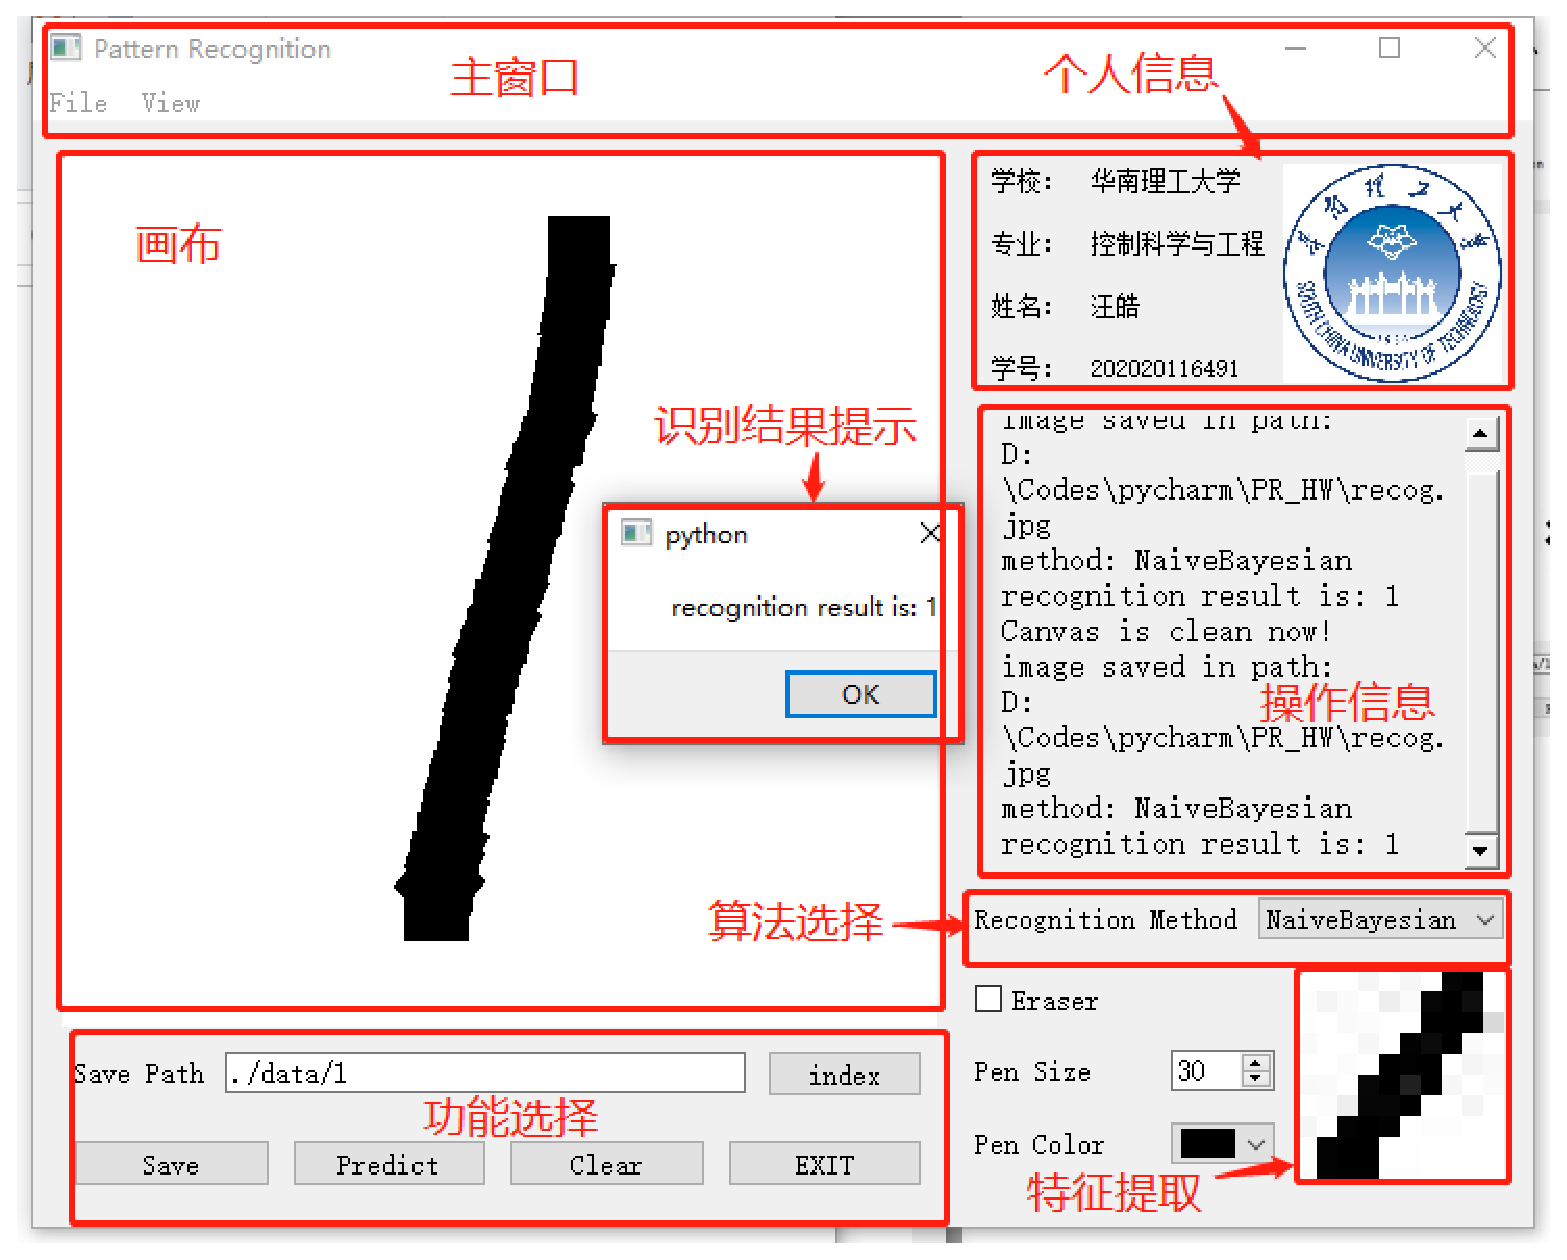
\includegraphics[scale=0.5]{./img/GUI.eps}
			\caption{GUI界面展示}
			\label{fig:2.2}
			\end{figure}	
\clearpage
\chapter{数据集}
	\section{数据集}
		利用GUI的画布手写数字,分为训练集和测试集,并按数字名存到文件夹中,文件目录如下所示。其中,训练集中每个数字有20张图片,测试集中每个数字有10张图片。
		\begin{figure}[!h]
			\centering
			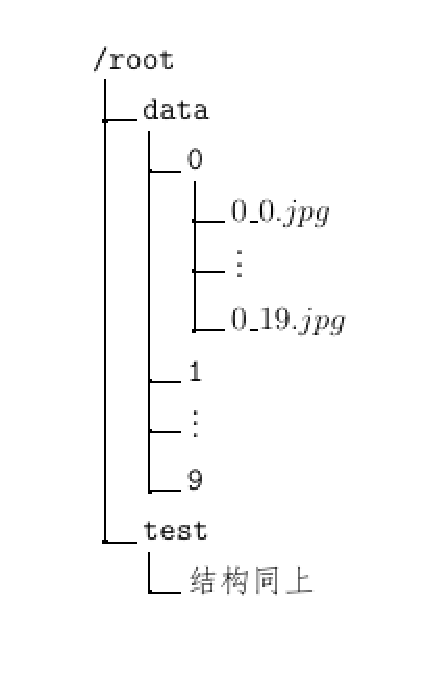
\includegraphics[scale=0.8]{./img/DataDirTree.eps}
			\caption{数据集文件目录}
			\label{fig:3.1}
		\end{figure}

	\section{特征处理}
		\subsection{目的}
			物理和结构上的特征通常易于为人的直觉感知,但有时难以定量描述,因而不易用于机器判别。而数学上的特征易于用机器定量描述和判别,故通常使用数学特征作为模式识别任务的特征描述,例如基于统计的特征。

			但对于一幅图像而言,例如我们的手写数字图像,尺寸是420*420,即使不考虑色彩,也至少有17万多个像素值作为原始特征。而每一个特征点的取值从0-255共有256个取值可能。原始这一幅图几十万的像素特征样本分布很稀疏,高维特征计算量大、冗余性高,且不能反映对象的本质。因而,特征处理的一个重要任务或目的就是从如此繁多的特征中选择其中的重要特征以减少特征数量,同时尽量保留分类信息。

		\subsection{处理方法}
			通常能够提取有效信息、压缩特征空间的特征处理方法有:特征提取和特征选择。所谓特征提取是用映射或变换的方法把原始特征变换为较少的新特征。而特征选择是指从原始特征中挑选出一些最有代表性、分类性能最好的特征。
		
			为了采用线性分类器中的Fisher,也就是LDA算法, 我们希望最后的特征满足以下条件:
			\begin{enumerate}[itemindent=1em]
				\renewcommand{\labelenumi}{\theenumi)}
				\item 每个特征之间尽量独立分布;
				\item 特征用一维数组表示;
				\item 特征取值尽量少;
				\item 特征数组维数尽量小。
			\end{enumerate}

			于是,我们将图像有效范围从420*420的像素阵中分割出来,设定阈值按均值滤波缩小到10*10或7*7,再转换成二值图,并展开成一维数组,最后得到一个尺寸为1*100维(或1*49维)的特征数组,其中间过程如图3.2所示。
			\begin{figure}[!h]
			\centering
			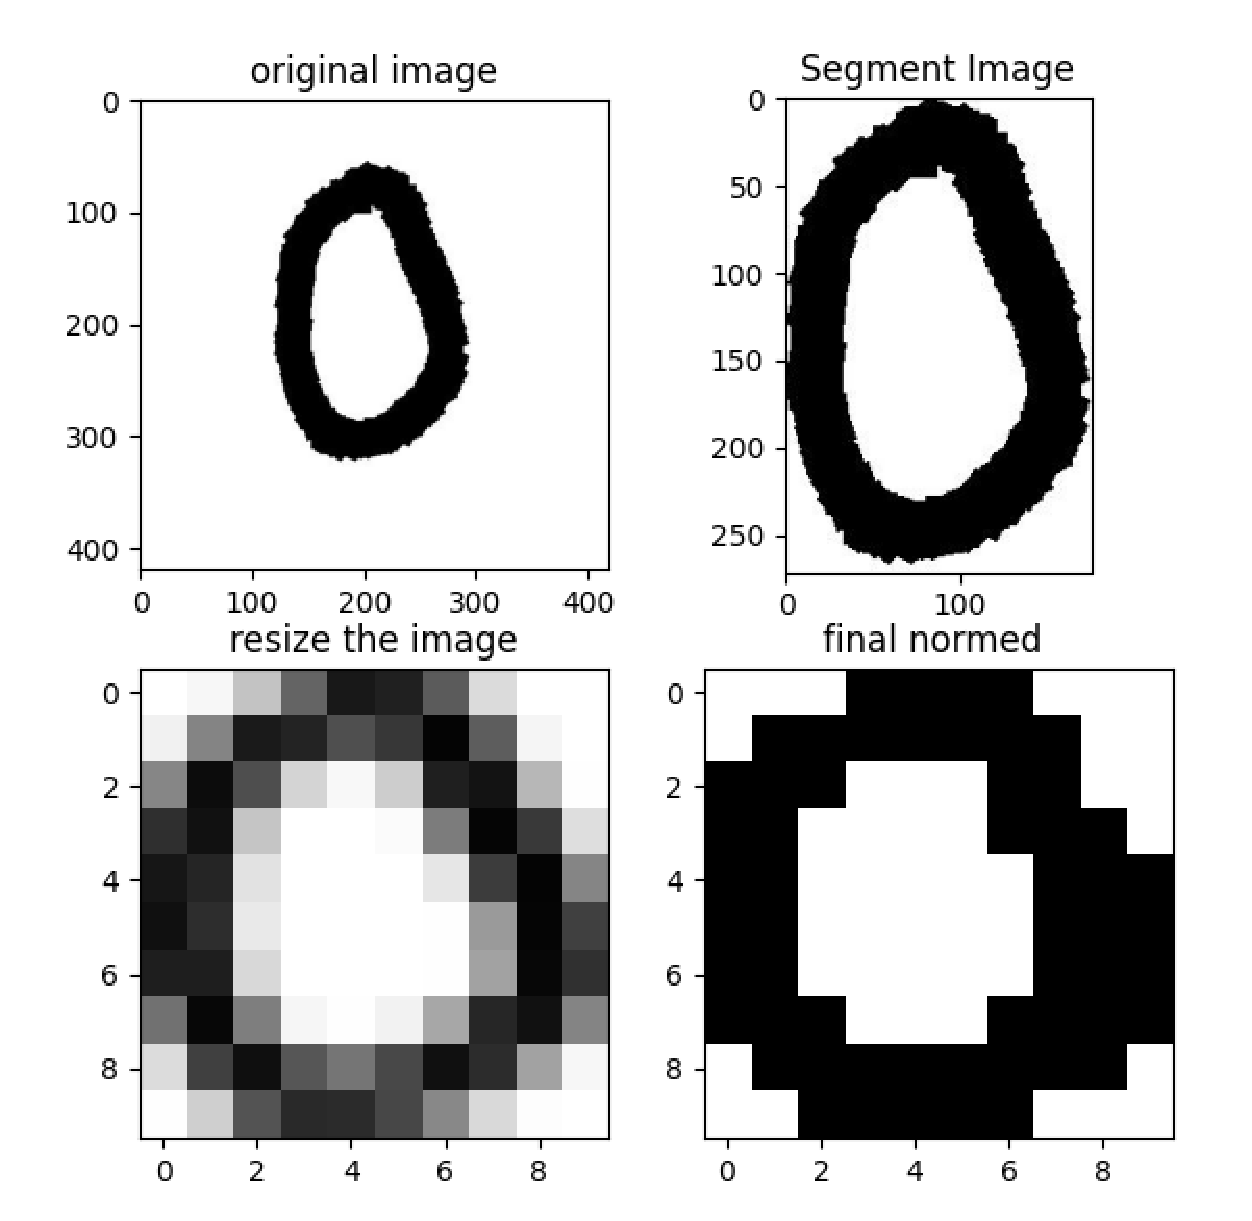
\includegraphics[scale=0.35]{./img/FeatureMapping.eps}
			\caption{特征处理过程}
			\label{fig:3.2}
			\end{figure}
\clearpage

\chapter{Fisher分类器}
	\section{二分类线性判别分析}
			线性判别分析是一种经典的线性学习方法,在二分类问题上因为最早由Fisher提出,故而亦称“Fisher”分类器。
		\subsection{BiFisher(二分类LDA)原理}
			LDA的思想非常朴素:给定训练样本集,设法将样本投影到一条直线上,使得同类样本的投影点尽可能接近、异类样本的投影点尽可能远离;在对新样本进行分类时,将其投影到同样的这条直线上,再根据投影点的位置来确定新样本的类别。

			给定数据集 $D=\{(\bm{x}_i, y_i)\}_{i=1}^{m}, y_i \in \{0, 1\}$,令 $X_i、\bm{\mu} _i、\Sigma_i$ 分别表示第 $i \in \{0, 1\}$ 类示例的集合、均值向量、协方差矩阵。若将数据投影到直线 $\bm{\omega}$ 上,则两类样本的中心在直线上的投影分别为 $\bm{\omega}^T\bm{\mu}_0$ 和 $\bm{\omega}^T\bm{\mu}_1$;若将所有样本点都投影到直线上,则两类样本的协方差分别为 $\bm{\omega}^T \bm{\Sigma}_0 \bm{\omega}$ 和 $\bm{\omega}^T \bm{\Sigma}_1 \bm{\omega}$。由于直线都是一维空间,故上述样本中心的投影和方差的投影都是实数。

			由于我们的目标是使同类样本的投影点尽可能近,故可以使同类样本投影点的协方差尽可能小,即 $\bm{\omega}^T \bm{\Sigma}_0 \bm{\omega}+\bm{\omega}^T \bm{\Sigma}_1 \bm{\omega}$ 尽可能小;而欲使异类样本的投影点尽可能远离,可以让类中心之间的距离尽可能大,即 $ \left\|\bm{\omega}^T \bm{\mu} _0 - \bm{\omega}^T \bm{\mu} _1\right\|_2^2 $ 尽可能大。于是,我们可以得到二分类线性判别分析的优化目标:
			\begin{equation}
			\begin{aligned}
				\max_{\bm{\omega}} \mathcal{J} &= \frac{ \left\|\bm{\omega}^T \bm{\mu} _0 - \bm{\omega}^T \bm{\mu} _1\right\|_2^2 }{\bm{\omega}^T \bm{\Sigma}_0 \bm{\omega}+\bm{\omega}^T \bm{\Sigma}_1 \bm{\omega}} \\
				&= \frac{\bm{\omega}^T (\bm{\mu}_0-\bm{\mu}_1)(\bm{\mu}_0-\bm{\mu}_1)^T \bm{\omega}}{\bm{\omega}^T(\Sigma_0+\Sigma_1)\bm{\omega}}
			\end{aligned}
			\end{equation}

			在此基础上我们定义“类内散度矩阵”和“类间散度矩阵”分别为:
			\begin{equation}
			\begin{aligned}
				\bm{S}_{\bm{\omega}} &= \Sigma _0 + \Sigma _1\\
				&= \sum_{\bm{x} \in X_0} {(\bm{x}-\bm{\mu} _0)(\bm{x} - \bm{\mu} _0)^T} + \sum_{\bm{x} \in X_1} {(\bm{x}-\bm{\mu}_1)(\bm{x}-\bm{\mu}_1)^T}
			\end{aligned}
			\end{equation}

			\begin{equation}
				\bm{S}_{\bm{b}} = (\bm{\mu}_0-\bm{\mu}_1)(\bm{\mu}_0-\bm{\mu}_1)^T
			\end{equation}

			于是,判别式4.1可改写成:
			\begin{equation}
				\bm{\omega} ^* = \max_{\bm{\omega}} \mathcal{J} = \frac{\bm{\omega}^T \bm{S}_{\bm{b}} \bm{\omega}}{\bm{\omega}^T \bm{S}_{\bm{b}} \bm{\omega}}
			\end{equation}

			观察上述判别式4.4,若令 $\bm{\omega}^T \bm{S}_{\bm{b}} \bm{\omega}=1$,则式4.4等价于:
			\begin{equation}
			\begin{aligned}
				&\min_{\bm{\omega}} -\bm{\omega}^T \bm{S}_{\bm{b}} \bm{\omega}\\
				&s.t. \bm{\omega}^T \bm{S}_{\bm{b}} \bm{\omega}=1
			\end{aligned}
			\end{equation}
再由拉格朗日法求解,得到二分类Fisher判别器的投影向量为:
			\begin{equation}
				\bm{\omega} ^* = \bm{S} _{\bm{\omega}}^{-1} (\mu_0-\mu_1)
			\end{equation}

		\subsection{VoteFisher(加权投票LDA)设计}
			考虑我们的手写数字识别任务属于多分类任务,故我们将其划分为多个二分类任务进行识别。考虑到最后加权的公平性,我们采用了加权投票法,其算法规则如下页算法1所示。
			\begin{algorithm}
			\caption{VoteFisher分类器} %算法的名字
			\hspace*{0.02in} {\bf Input:} %算法的输入, \hspace*{0.02in}用来控制位置,同时利用 \\ 进行换行
			训练集和测试集数据 $D=\{(\bm{x}_i, y_i)\}_{i=1}^{m}, y_i \in \{0, 1, \cdots, 9\}$ \\
			\hspace*{0.02in} {\bf Train:}
			\begin{algorithmic}[1]
			\State 加载训练集数据,计算数据可能的类别数 $N=10$,并将数据集按类别分成10堆; % \State 后写一般语句
			\For{$i=0:9$} % For 语句,需要和EndFor对应
				\For{$j=0:9$} % For 语句,需要和EndFor对应
					\State 计算总数据的均值 $\mu$;
					\State 加载训练集并计算第 $i$ 类和第 $j$ 类数据的均值 $\mu_i, \mu_j$ 和方差 $\Sigma_i, \Sigma_j$;
					\State 根据式4.2和4.3计算类内散度 $\bm{S}_{\bm{\omega}}$ 和类间散度 $\bm{S}_{\bm{b}}$;
					\State 根据式4.6计算投影面的权重 $\bm{\omega} $;
					\State 计算投影空间里第 $i$ 类和第 $j$ 类数据的中心 $c_i$ 和 $c_j$;
					 \State 加载测试集数据,将其中属于第 $i$ 类和第 $j$ 类的数据喂到训练好的 $i-j$ 分类器中,计算其训练准确度 $v$;
					\State 将投影面权重 $\bm{\omega} $、投影中心 $c_i$ 和 $c_j$以及训练准确度 $v$ 返回作为 $i-j$ 分类器的参数;
				\EndFor
			\EndFor
			\end{algorithmic}
			\hspace*{0.02in} {\bf Test:}
			\begin{algorithmic}[1]
			\State 设置投票箱 $vote=torch.zeros((10, ))$;
			\State 加载测试集数据;
			\For{$i=0:9$} % For 语句,需要和EndFor对应
				\For{$j=0:9$} % For 语句,需要和EndFor对应
					\State 计算测试图片 $\bm{x}$在投影面上的投影 $p = \bm{\omega}^T \bm{x}$;
					\State 计算其到两中心店之间的距离 $d_i$ 和 $d_j$;
					\If{$d_i < d_j$} % If 语句,需要和EndIf对应
						\State $vote[i] += v$
					\Else
						\State $vote[j] += v$
					\EndIf
				\EndFor
			\EndFor
			\State \Return vote
			\end{algorithmic}
			\hspace*{0.02in} {\bf Output:} %算法的结果输出
			各类别的投票
			\end{algorithm}

			这里,我们为了保证公平性,设置了10*10一共100个分类器,而对于每两类之间我们做一个分类器,每十个分类器作为一个类别的分类器集,进行投票选择。其实亦可以采用45个分类器,但设计时考虑书写简便,直接设置了100个分类器。

		\subsection{VoteFisher实现}
			我们在 $pytorch$ 中实现上述算法,采用 $numpy$ 和 $pytorch$ 库使用 $CPU$ 对其矩阵计算进行加速,最后得到一个集成的投票二分类Fisher分类器。为了评价我们的系统,我们取测试集的所有图片进行预测,然后计算其 $top1$ 和 $top5$ 准确率分别为 $68\%$ 和 $97\%$。显然其 $top1$ 准确度比较低。

	\section{多分类LDA}
		\subsection{MultiFisher(多分类LDA)原理}
			承接上述BiFisher的内容,将LDA拓展到多分类任务中。假定存在 $N$ 个类,且第 $i$ 类示例数为 $m_i$,在此基础上我们定义三个“散度矩阵”。
			\begin{enumerate}[itemindent=1em]
				\renewcommand{\labelenumi}{\theenumi)}
				\item 全局散度矩阵:
					\begin{equation}
					\begin{aligned}
						\bm{S}_{\bm{t}} &= \bm{S}_{\bm{b}} + \bm{S}_{\bm{\omega}}  \\
						&=\sum_{i=1}^{m} (\bm{x}_i - \bm{\mu}) (\bm{x}_i - \bm{\mu})^T
					\end{aligned}
					\end{equation}
				\item 类内散度矩阵:
					\begin{equation}
					\begin{aligned}
						\bm{S}_{\bm{\omega}} &= \sum_{i=1}^{N} {\bm{S}_{\bm{\omega}_i}}  \\
						&=\sum_{i=1}^{N} {\sum_{\bm{x} \in \bm{X}_i} {(\bm{x} - \bm{\mu}_i) (\bm{x} - \bm{\mu}_i)^T}}
					\end{aligned}
					\end{equation}
				\item 类间散度矩阵:
					\begin{equation}
					\begin{aligned}
						\bm{S}_{\bm{\omega}} &= \bm{S}_{\bm{t}} - \bm{S}_{\bm{\omega}}  \\
						&=\sum_{i=1}^{N} {m_i (\bm{\mu}_i - \bm{\mu}) (\bm{\mu}_i - \bm{\mu})^T}
					\end{aligned}
					\end{equation}
			\end{enumerate}

			故而,多分类Fisher的优化目标可写成:
			\begin{equation}
				\bm{W} ^* = \max_{\bm{W}} \mathcal{J} = \frac{tr(\bm{W}^T \bm{S}_{\bm{b}} \bm{W})}{tr(\bm{W}^T \bm{S}_{\bm{b}} \bm{W})}
			\end{equation}
由拉格朗日可求得 $\bm{W}$ 满足下式:
			\begin{equation}
				\bm{S}_{\bm{b}} \bm{W} = \lambda \bm{S}_{\bm{\omega}} \bm{W}
			\end{equation}
由上式,显然 $\bm{W}$ 的闭式解是矩阵 $\bm{S}_{\bm{\omega}}^{-1} \bm{S}_{\bm{b}}$的广义特征向量。
		\subsection{设计}
			在实际计算中,以我们的手写数字任务为例,即使我们对输入图片做前述特征提取,特征依然有冗余,且维度较高(10*10的特征维度有100维)。而在实际求解 $\bm{S}_{\bm{\omega}}^{-1} \bm{S}_{\bm{b}}$的广义特征值时发现,部分特征值较小或为0,只有部分特征值较大,在很大程度上代表了原矩阵的特征,而其他较小特征值则更多的是包含了图片的特异性信息和噪声信息,对我们的训练任务没有任何帮助。故而我们可以通过计算特征值将 $\bm{W}$ 维度降到 $N-1$ 维,为了确保算法的准确性,这里我提取了前 $dim(\bm{x})/2$个最大特征值对应的特征向量。 其算法如下:
			\begin{algorithm}
			\caption{MultiFisher分类器} %算法的名字
			\hspace*{0.02in} {\bf Input:} %算法的输入, \hspace*{0.02in}用来控制位置,同时利用 \\ 进行换行
			训练集和测试集数据 $D=\{(\bm{x}_i, y_i)\}_{i=1}^{m}, y_i \in \{0, 1, \cdots, 9\}$ \\
			\hspace*{0.02in} {\bf Train:}
			\begin{algorithmic}[1]
			\State 加载训练集数据,计算数据可能的类别数 $N=10$,并将数据集按类别分成10堆; % \State 后写一般语句
			\State 计算总数据的均值 $\mu$与各类的均值 $\mu_i$ ;
			\State 根据式4.8和4.9计算类内散度 $\bm{S}_{\bm{\omega}}$ 和类间散度 $\bm{S}_{\bm{b}}$;
			\State 计算 $\bm{S}_{\bm{\omega}}^{-1} \bm{S}_{\bm{b}}$的广义特征值和特征向量;
			\State 将特征值从大到小排列,取前 $N-1$ 个对应的特征向量作为  $\bm{\omega}$;
			\State 计算投影面上的各类中心 $c_i$;
			\State \Return   $\bm{\omega}$、$c_i$。
			\end{algorithmic}
			\hspace*{0.02in} {\bf Test:}
			\begin{algorithmic}[1]
			\State 输入特征提取后的图片特征 $\bm{x}$;
			\State 计算图片特征在投影面上的投影 $p = \bm{W}^T \bm{x}$;
			\State 计算投影到各类中心的距离 $d_i$;
			\end{algorithmic}
			\hspace*{0.02in} {\bf Output:} %算法的结果输出
			各类别的距离
			\end{algorithm}

		\subsection{实现}
			在 $python$ 中,使用 $pytorch$ 利用 $CPU$ 对矩阵计算加速。在求 $\bm{S}_{\bm{\omega}}^{-1} \bm{S}_{\bm{b}}$ 时,由于求逆比较麻烦,求伪逆亦比较麻烦,故采用正交分解 $\bm{S}_{\bm{\omega}} = U diag(\Lambda) V$,于是 $\bm{S}_{\bm{\omega}}^{-1} = U^T diag(\Lambda ^{-1}) V^T$,从而减小了计算难度,最后得到一个MultiFisher分类器。

			为了评价我们的系统,我们取测试集的所有图片进行预测,然后计算其 $top1$ 和 $top5$ 准确率分别为 $87.5\%$ 和 $100\%$。

	\section{算法评价}
		由于我们自己设计的Fisher算法的准确率并不是很高,故我们特意选取了 $sklearn$ 库里面 $LinearDiscriminantAnalysis$ 函数进行对比,对比结果如下表所示。虽然我们设计的分类器较标准分类器之间仍有不少差距,但从结果看,我们所设计的分类器还是能够很好的完成任务。

		\begin{table}[!h]
		\centering
		\caption{Fisher训练器top1和top5准确率对比}  
		\begin{tabular*}{8cm}{lll}  
		\hline  
		算法 & top1(\%)  & top5(\%) \\  
		\hline  
		\hline
		VoteFisher  & 68 & 97 \\  
		MultiFisher  & 87.5 & 100 \\  
		SkLearn-Fisher5 & 95 & 100\\
		\hline  
		\end{tabular*}  
		\end{table}  
\clearpage

\chapter{实验结果与结论}
	我们将保存的算法模型导入 $GUI$ 对应的预测函数中,进行测试,如图5.1-图5.3所示。当分别选择了VoteFisher、MultiFisher和SklearnFisher作为预测算法进行预测,在正常书写时均能准确预测出正确结果,并能在 $GUI$ 右下角反映出特征提取后的可视化图形。而预测结果及其他信息则能通过右边的信息框反映出来,同时预测结果以弹窗的形式反映。

		经过多次测试,发现所设计的三种Fisher分类器均能够很好地完成手写数字分类任务。

		\begin{figure}[!h]
		\centering
		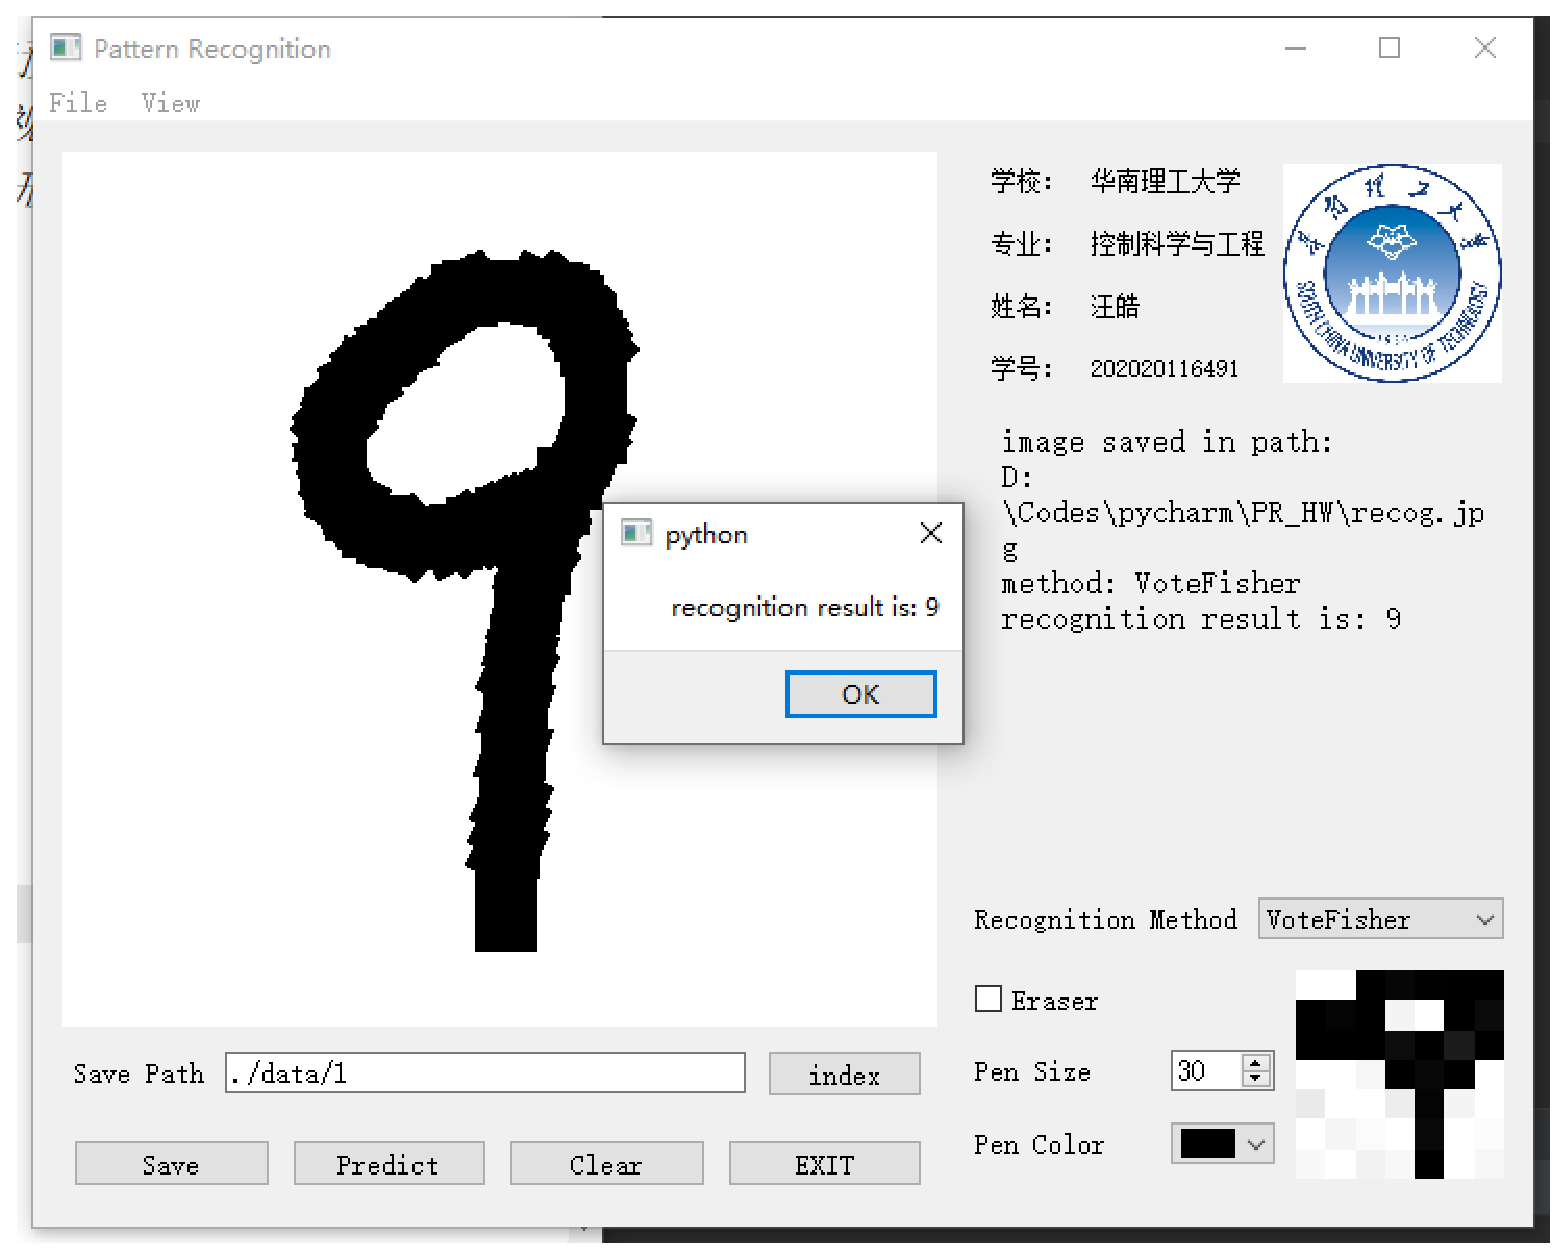
\includegraphics[scale=0.4]{./img/Predict1.eps}
		\caption{VoteFisher预测结果展示}
		\label{fig:5.1}
		\end{figure}
		\begin{figure}[!h]
		\centering
		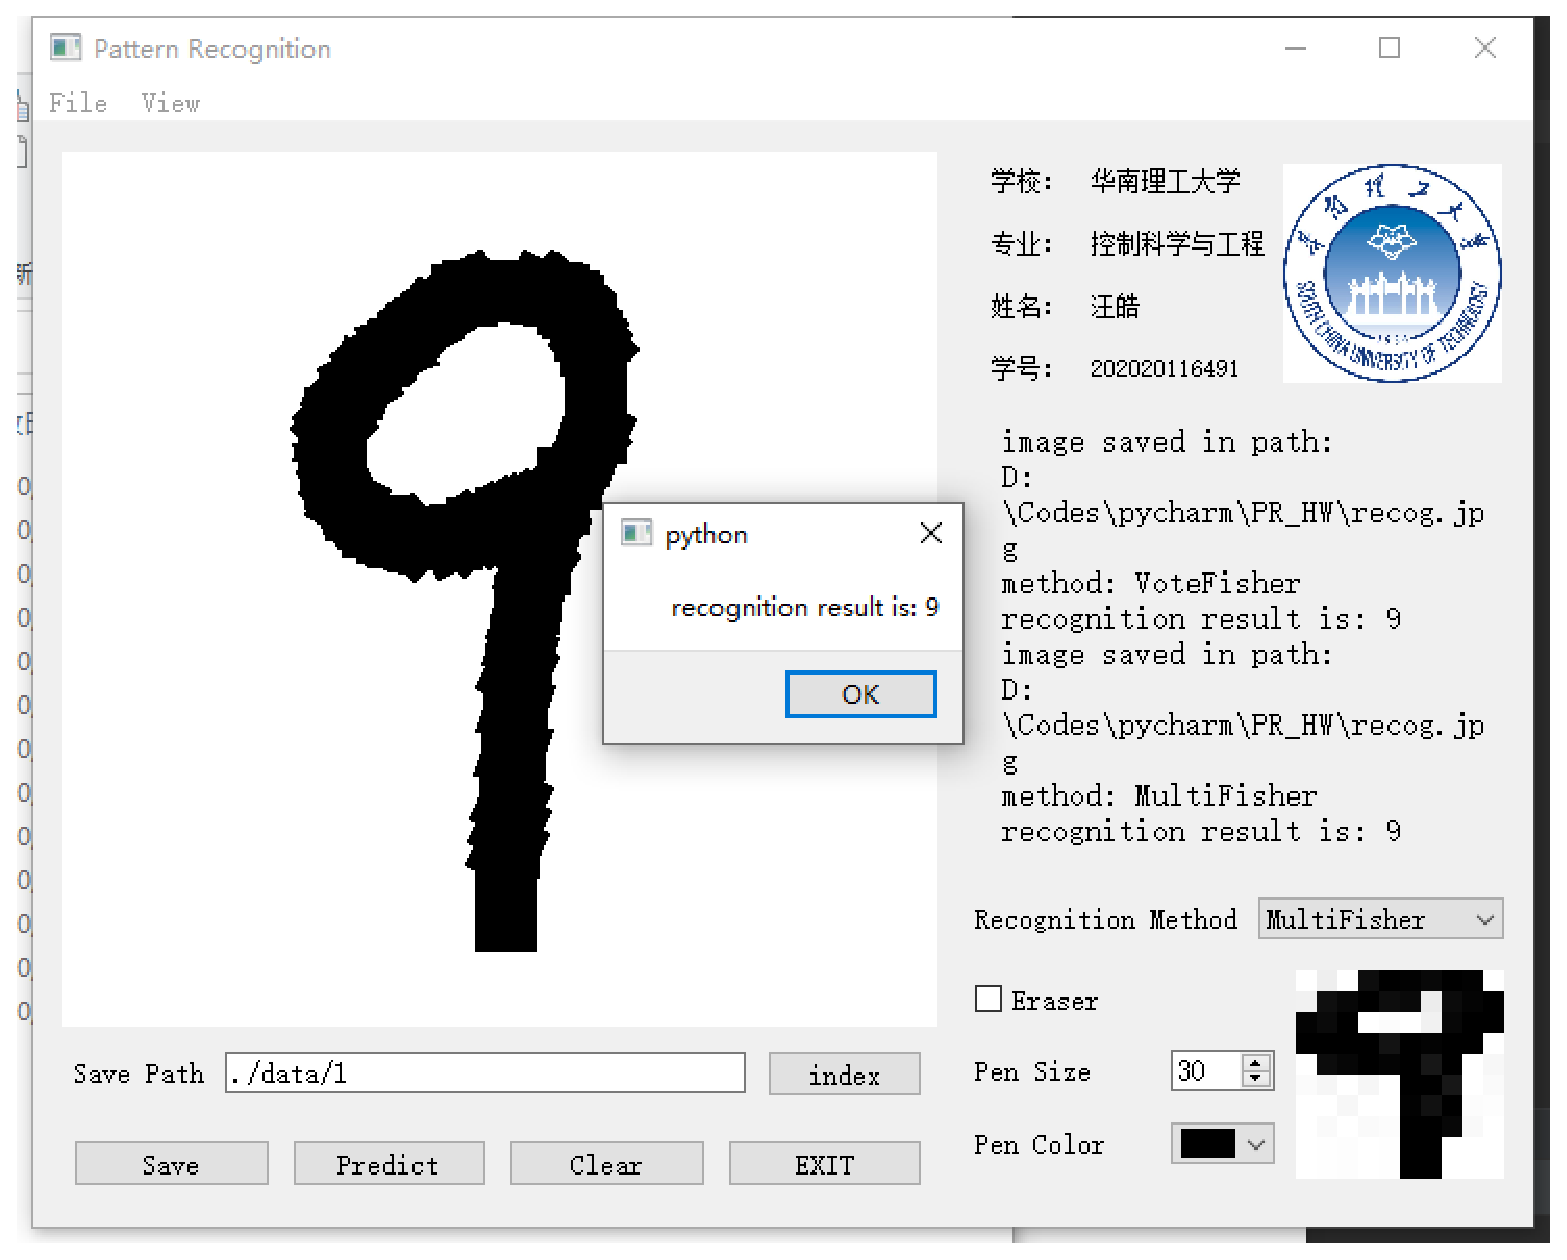
\includegraphics[scale=0.4]{./img/Predict2.eps}
		\caption{MultiFisher预测结果展示}
		\label{fig:5.2}
		\end{figure}
		\begin{figure}[!h]
		\centering
		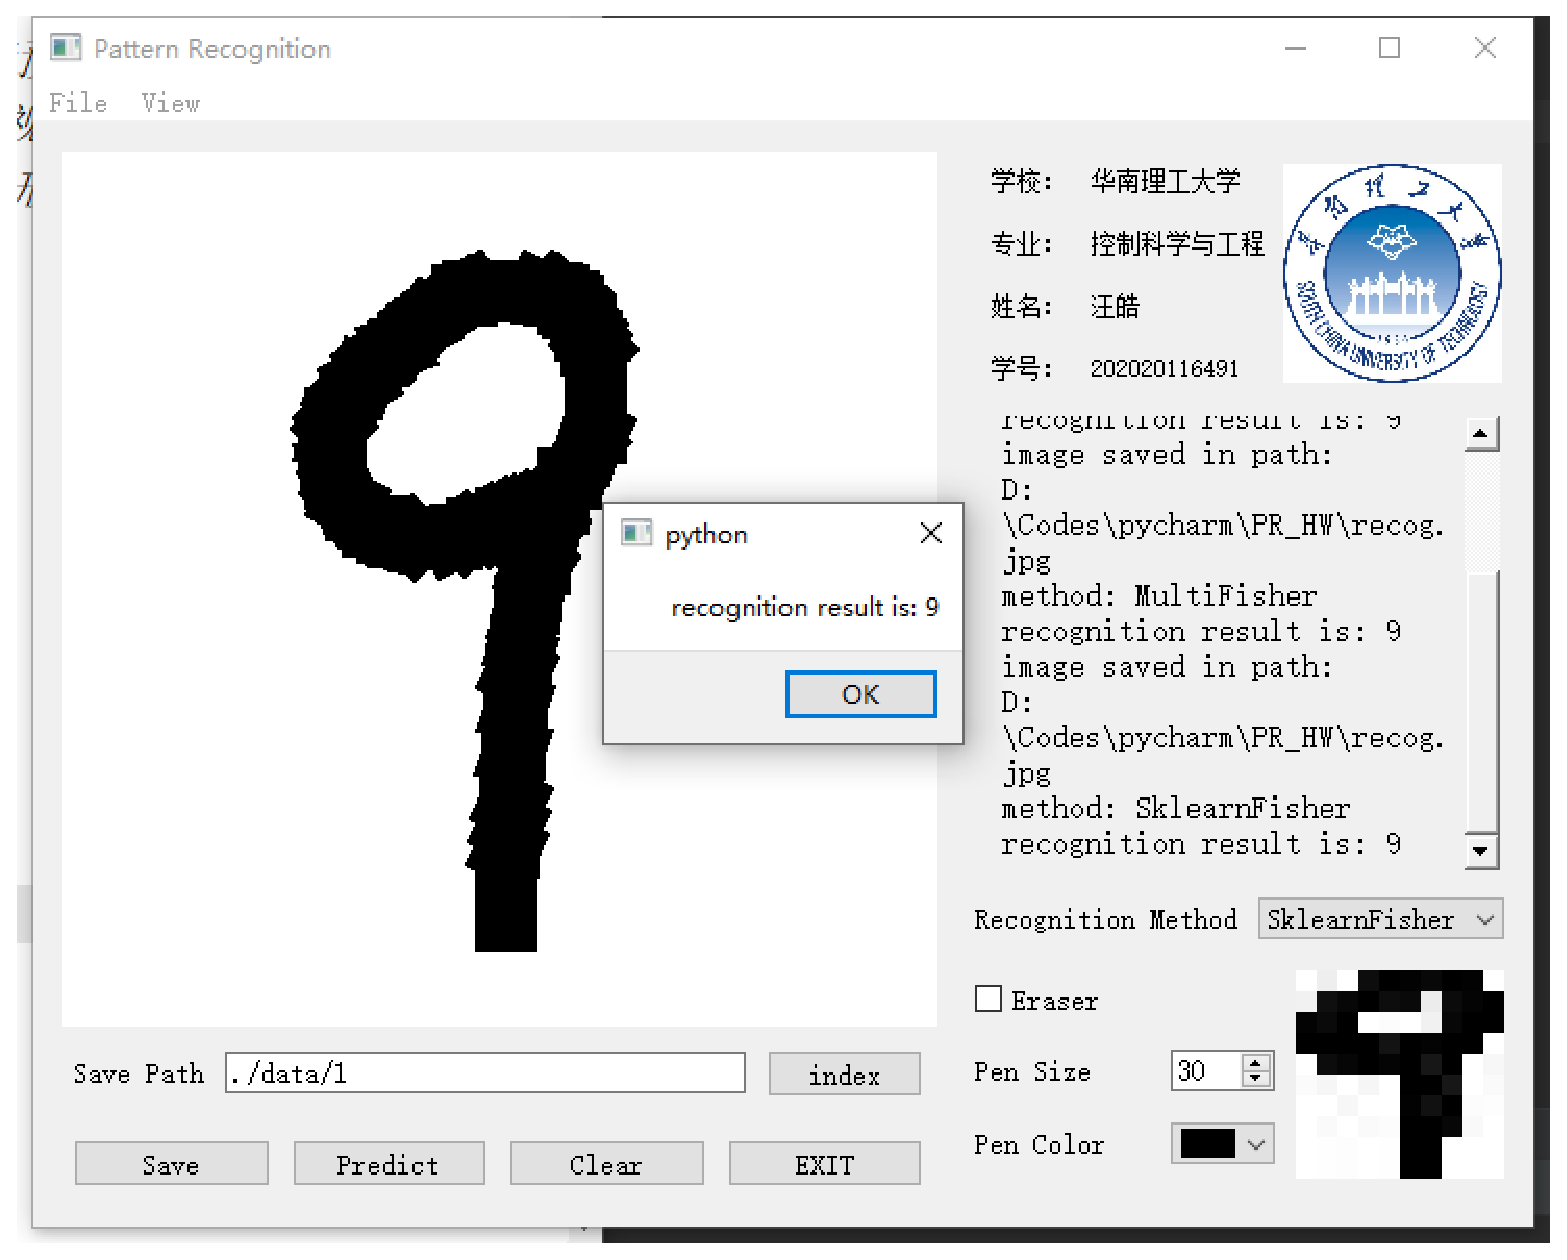
\includegraphics[scale=0.4]{./img/Predict3.eps}
		\caption{SklearnFisher预测结果展示}
		\label{fig:5.3}
		\end{figure}

\clearpage
\end{document}